

Following \citet{jiao2017} I define the network measurments and the expected direction of their effect


\subsubsection{Density effect (Edges)}

Density refers to the proportion of connections in a social network relative to the total possible connections.

This is interpreted as the intercept of the model. The entry of the `density` matrix $M_{ij}$ 
indicates how the presence of that edge changes the number of edges in the graph, holding the 
rest of the network constant. It a matrix of ones - with the upper right triangle masked in the 
case of undirected networks.

\subsubsection{Small-World effect (Triangles)}

Social networks tend to exhibit a much higher number of triangles and transitive triads than what 
would be predicted by random graphs with comparable density.

Triangles, which represent a set of three documents or concepts who are mutually connected, are a common feature of social networks and are thought to play an important role in social cohesion and network structure \citep{kossinets2006, newman2018}.

The entry of the triangle matrix $M_{ij}$ indicates how the presence of that edge changes the number of triangles in the graph, holding the rest of the network constant. 

Overall tendency of networks to be composed of local densities (closure). Are the ties randomly distributed of do they form local structures.A graph with a low triangle effect would look homogeneous distribution of substructures is what we would expect from a random graph

Lumps appear (local structures)

\subsubsection{Closure effect (Transitivity)}

A triad is a group of three nodes in a graph. A triad can either be open or closed. An open triad is a group of three nodes that are connected by two edges (Figure \ref{fig:open_triad}), while a closed triad is a group of three nodes that are connected by three edges (Figure \ref{fig:closed_triad}). 

\begin{figure}[H]
    \centering
    \begin{subfigure}[t]{0.4\textwidth}
        \centering
        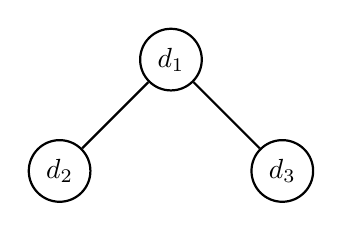
\begin{tikzpicture}[node distance=2cm, thick, main/.style = {draw, circle}]
            \node[main] (1) [] {$d_1$};
            \node[main] (2) [below left of=1] {$d_2$};
            \node[main] (3) [below right of=1] {$d_3$};
            \draw[] (1) to (2);
            \draw[] (1) to (3);
        \end{tikzpicture}
        \caption{Open Triad} 
        \label{fig:open_triad}
     \end{subfigure}
        ~
     \begin{subfigure}[t]{0.4\textwidth}
        \centering
        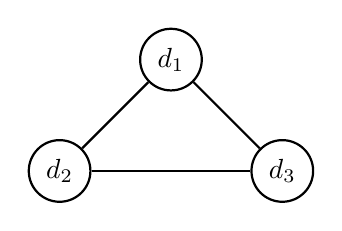
\begin{tikzpicture}[node distance=2cm, thick, main/.style = {draw, circle}]
            \node[main] (1) [] {$d_1$};
            \node[main] (2) [below left of=1] {$d_2$};
            \node[main] (3) [below right of=1] {$d_3$};
            \draw[] (1) to (2);
            \draw[] (1) to (3);
            \draw[] (2) to (3);
        \end{tikzpicture}
        \caption{Closed Triad} 
        \label{fig:closed_triad}
     \end{subfigure}
     \caption{Triads}
\end{figure}

Transitivity is defined as the ratio of the number of closed triads in the graph to the number of open triads in the graph.

$$
T = \frac{3t_c}{t_o}
$$

Where $t_c$ is the number of closed triads and $t_o$ is the number of open triads.


\subsubsection{Clique effect (Cliques)}

Tendecy for there to be parts of the graph where multiple nodes all co-occur more than by random change

If I discuss 
A all other concepts in the clique it belongs to.
highly related to each other distinct topical or functional units within the network

This build on triangles (which are a clique) but captures more information 

It asks whether triangles overlap to form larger structurees rather than just isolated (random) triangles

Densly connected always connected

\subsubsection{Silo effect (Components)}

silos refer to isolated areas of research or knowledge that are not well connected to other areas or fields limit the flow of information and influence within the network
Hyper specialization of field of knowledge
Talk to one another but never talk to nodes outside their primary group

\subsubsection{Popularity effect ($k$-star)}

The popularity effects in most classes were not obvious, which meant the degree (the total number of actors selecting an individual) of individuals in the class networks had little difference.

\begin{figure}[H]
    \centering
    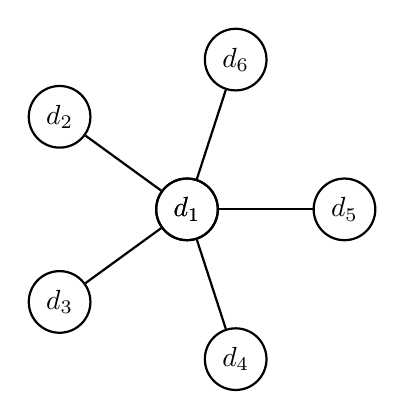
\begin{tikzpicture}[node distance=2cm, thick, main/.style = {draw, circle}]
        \node[main] (1) at (360:0mm) (center) {$d_1$};
        \node[main] (1) [] {$d_1$};
        \foreach \n in {2,...,6}{
            \node[main] at ({\n*360/5}:2cm) (n\n) {$d_\n$};
            \draw (center)--(n\n);
        }
    \end{tikzpicture}
    \caption{Star} \label{fig:k_star}
\end{figure}

What we mean by a strong k star effect
Control for 9 stars in order to determine if 10 star is significant
10 star is a bunch of 9 stars

\subsubsection{Mediating effect (betweenness centrality)}

Nodes with high betweenness centrality in this type of network may represent important bridge terms or pivot terms that connect different topics or themes within the corpus of documents. The betweenness centrality $c_b$ of node $n$ is given by:

$$
c_b(i) = \sum_{j \ne k} \frac{\sigma_{jk}(i)}{\sigma_{jk}}
$$

Where $\sigma_{ij}$ is the total number of shortest paths from node $i$ to node $j$ and $\sigma_{ij}(n)$ is the number of those paths that pass through node $n$. In other words, it is the proportion of all shortest paths between nodes $i$ and $j$ that pass through node $n$. The average betweenness centrality over all nodes of the network is taken as another network statistic. 

Indicates good integration but maybe structural fragility (if central nodes are removed, speperate components)

\subsubsection{Community effect (Louvain)}

The Louvain community detection method consists of two main steps. Initially, each node is assigned to a separate community. Then, for each node, the algorithm attempts 
to optimize the modularity of the network by evaluating the potential gain in modularity achieved by 
moving the node to each of its neighboring communities. If no gain is achieved, the node remains in 
its original community.

In the second step, a new network is constructed where each node represents a community from the 
previous step. The edges between the new nodes are weighted by the sum of the weights of the edges 
between the nodes in the corresponding communities in the original network. The Louvain method is then 
applied to this new network, and the process is repeated until no further improvement in modularity 
can be achieved.

Modularity is a measure of the degree of segregation of a network into communities. It is calculated 
as the difference between the fraction of edges within a given group and the expected fraction of 
edges if they were randomly distributed in the network. The change in modularity $\Delta Q$ achieved 
by moving the node to each of its neighboring communities is measured as

$$
Q = \frac{1}{2m}\sum_{i,j}[A_{ij} - \frac{k_ik_j}{2m}]\delta(c_i,c_j)
$$

where:
\begin{itemize}
    \item $Q$ is the modularity index
    \item $m$ is the total number of edges in the network
    \item $A_{ij}$ is the weight of the edge between nodes $i$ and $j$
    \item $k_i$ and $k_j$ are the degrees of nodes $i$ and $j$, respectively
    \item $c_i$ and $c_j$ are the community assignments of nodes $i$ and $j$
    \item $\delta(c_i,c_j)$ is the Kronecker delta, which is equal to 1 if nodes $i$ and $j$ are in the same community and 0 otherwise.
\end{itemize}

% \subsection{Importance effect (closeness)}

% Nodes with high closeness centrality in these networks may represent important key concepts or core ideas that are central to the understanding of the corpus of documents or, conversly, those that constitute the periphery within the network and are relatively more isolated. On a graph of $n$ nodes, closeness centrality is defined as

% $$
% c_c(i) = \frac{n - 1}{\sum\limits_{i \ne j} d(i, j)}
% $$

% Where $d(i,x)$ is the distance (length of the shortest path) between nodes $i$ and $y$. The average closeness centrality over all nodes of the network is taken as another network statistic. 

% Integration of the field
% Concepts play integrating
% Separated by few or many logical steps

% \subsection{Community centrality (Eigenvector)}

% Eigenvector centrality is a network measure that assigns a score to each node in a network based on the node's connections to other high-scoring nodes. This measure takes into account not only the number of connections a node has, but also the quality or importance of those connections. The average closeness centrality over all nodes of the network is taken as another network statistic.


% \subsection{Concentration effect (Centralization)}

% Measure of the degree of concentration of edges. Centralization is obtained by computing the ratio of the differences between the highest scoring node and all other nodes for both the observed and a star network of the same size.

% $$
% D(G) = \sum_i (max(c) - c_i)
% $$

% where $c_i$ is the centrality $c$ of node $i$ and $max(c)$ is the largest centrality score in graph $G$.  by the maximum theoretical score for a graph with the same number of vertices:

% $$
% C(G) = \frac{D(G)}{D(G_{star})}
% $$


% \subsection{Inequality effect (Gini coefficient)}


% The Gini coefficient in a network can be defined as the ratio between the area between the Lorenz curve and the line of perfect equality ($A$) to the area under the line of perfect equality ($A + B$). The line of perfect equality is a straight line that represents a situation in which all nodes has the same number of edges. The Lorenz curve plots the cumulative proportion of edges against the cumulative proportion of nodes.

% $$
% G = \frac{A}{A + B}
% $$

% As $A$ grows relative to $B$, the fraction tends towards 1, indicating perfect inequality. Conversely, As $B$ grows raltive to $A$, the faction tends towards 0, indicating perfect equality.

% \subsection{Geodesic distance}

% To calculate the average geodesic distance, the shortest path length between every pair of nodes 
% is first computed, and then the average of all these distances is taken. The result is a single value 
% that represents the typical distance between any two nodes in the graph.

